% =====================================================================
%  CSC_43M04_EP — Computer Vision with Deep Learning (École Polytechnique)
%  Team 8 — Florian Guillaumey & Andrea Signoretti
%  Report v2: unified two-track report (Closed World + Open World).
%
%  CVPR double-column template. Requires cvpr.sty + ieeenat_fullname.bst
%  (already in docs/). silence.sty and cleveref.sty stubs are provided for
%  TeX installs that lack them.
%
%  Build (from docs/):
%    export TEXINPUTS="$PWD:" BSTINPUTS="$PWD:" BIBINPUTS="$PWD:"
%    pdflatex report_cvpr_v2 && bibtex report_cvpr_v2 && pdflatex report_cvpr_v2 && pdflatex report_cvpr_v2
%
%  Figures live in docs/figures/ and are gathered at the END after \clearpage.
% =====================================================================
\documentclass[10pt,twocolumn,letterpaper]{article}

\usepackage{cvpr}              % final (camera-ready) mode
\usepackage{graphicx}
\usepackage{amsmath,amssymb}
\usepackage{booktabs}
\usepackage{xcolor}
\usepackage[pagebackref,breaklinks,colorlinks,allcolors=blue]{hyperref}

\graphicspath{{figures/}}

\def\cvprPaperID{8}
\def\confName{CSC\_43M04\_EP — Modal d'informatique}
\def\confYear{2026}

\title{What Happens Next? Closed- and Open-World Video Action Recognition\\
on a 33-Class Something-Something\,V2 Subset}

\author{%
Florian Guillaumey\\
École Polytechnique --- Team 8\\
{\tt\small florian.guillaumey@polytechnique.edu}
\and
Andrea Signoretti\\
École Polytechnique --- Team 8\\
{\tt\small andrea.signoretti@polytechnique.edu}
}

\begin{document}
\maketitle
\thispagestyle{plain}
\pagestyle{plain}
\vspace{-1.2em}
\begin{center}\small May 27, 2026\end{center}

% =====================================================================
\begin{abstract}
We present a two-track study of temporal action prediction on a 33-class subset
of Something-Something\,V2 (SSv2)~\cite{goyal2017ssv2}, ``What Happens Next?'':
only the first ${\approx}40\%$ of each clip (four JPEG frames) is given, so the
outcome is withheld and classification must reason about motion. In
\textbf{Track~A (Closed World)}, where pretraining is forbidden, two data-centric
fixes dominate architecture: a 10-epoch \emph{regularisation warm-up}
($+36.3$\,pp) and matching the model's frame count to the true clip length
($+4.4$\,pp, beating a $3\times$ parameter scale-up). A log-softmax ensemble of
Temporal-Shift-Module~\cite{lin2019tsm} and CNN--Transformer models with
test-time augmentation reaches \textbf{44.03\%} top-1 on the official validation
set. In \textbf{Track~B (Open World)}, we fine-tune
V-JEPA\,2~\cite{bardes2025vjepa2} and VideoMAE~\cite{tong2022videomae} backbones
with progressive unfreezing, layer-wise learning-rate decay, window-capped
source-frame re-extraction and pseudo-labelling, then build a 14-model uniform
ensemble reaching \textbf{0.6586} Kaggle top-1 (16th in both tracks). We document
a self-discovered data-leakage event (a discarded 0.81 submission) and show that
ensemble diversity across architecture families beats single-family or
learned-weight ensembling. Failure analysis attributes the residual errors to
real-vs-pretended and direction-ambiguous classes that four frames
under-determine.
\end{abstract}

% =====================================================================
\section{Problem Description}
\label{sec:problem}

\paragraph{Task.}
The challenge classifies four-frame JPEG clips into one of 33 motion-defined
action classes (e.g.\ \emph{Pouring something into something}, \emph{Pulling
something from left to right}). Crucially, each clip contains only the
\emph{anticipatory} portion of the source SSv2 video---the shipped
\texttt{frame\_003} sits at a median fraction of $0.40$ of the source clip---so
the action's outcome is deliberately withheld and the task probes motion
prediction, not final-state recognition~\cite{goyal2017ssv2}.

\paragraph{Dataset.}
The split provides $44{,}993$ training clips, $6{,}745$ validation clips and
$6{,}913$ test clips over 33 classes (numeric prefixes 000--032; class~027 is
absent from training). Classes are heavily imbalanced: the largest (009,
\emph{Moving something up}) has $3{,}170$ examples while the smallest (026,
\emph{Spilling something next to something}) has only 162, a ratio of
$19.6\times$. The KL divergence between training and validation class
distributions is $0.088$, confirming the splits are representative.

\paragraph{Evaluation and tracks.}
Submissions are scored by top-1 accuracy on a public+private Kaggle leaderboard
over two stages (Stage~1, intermediate; Stage~2, final); top-5 is tracked
internally. The provided baseline reaches ${\approx}0.55$ private and the
second-place public reference is $0.74$; our final submissions placed
\textbf{16th in both tracks} (counting the multiple accounts fielded by some
teams). Following the challenge, we report two regimes. \textbf{Track~A (Closed World)} prohibits pretrained
models and external data---all spatial features, temporal dynamics and class
boundaries are learned from scratch on the four provided frames. \textbf{Track~B
(Open World)} permits pretrained backbones and external corpora but not future
frames or test labels. The task is hard for three reasons: (i)~labels are
motion-defined, defeating appearance-only models~\cite{goyal2017ssv2}; (ii)~four
frames is an order of magnitude below the 8--32 standard in video
recognition~\cite{lin2019tsm,bertasius2021timesformer}; (iii)~the discriminative
cue---the action's outcome---is withheld by construction.

% =====================================================================
\section{Methods}
\label{sec:method}

\subsection{Track A --- Closed World}
\label{sec:trackA}
The pipeline evolved through six iterations on an internal training-split, all
trained from scratch. Our guiding hypothesis is that, without pretraining,
\emph{every parameter spent on temporal modelling is one not spent learning
spatial features}, favouring parameter-free temporal mechanisms over heavy
temporal heads.

\subsubsection{Architecture family}
A ResNet-18~\cite{he2016resnet} with temporal average-pooling
(\textbf{CNNBaseline}) and a per-frame-feature \textbf{CNN-LSTM} serve as lower
bounds; with four frames the LSTM gives only marginal gains because
backpropagation through time on such short sequences is unstable.
\textbf{VideoFormer-Lite (VFL)} passes per-frame ResNet-18 features and a
learnable \texttt{[CLS]} token~\cite{dosovitskiy2021vit} through a 2-layer
pre-norm Transformer encoder~\cite{xiong2020prenorm} (global temporal attention
over the four tokens) and classifies the \texttt{[CLS]} representation,
reaching $53.37\%$ internal; it is a lightweight relative of
TimeSformer~\cite{bertasius2021timesformer} that keeps a CNN spatial encoder
for sample-efficiency from scratch.
\textbf{TSM-ResNet}~\cite{lin2019tsm} wraps every residual block of ResNet-18:
$1/\text{fold\_div}$ of channels are shifted one step backward and another
$1/\text{fold\_div}$ one step forward along the time axis, mixing temporal
information at \emph{zero parameter cost} by re-indexing tensor slices.
TSM was designed for SSv2-style motion labels and is therefore a strong prior
here (Fig.~\ref{fig:arch}); the two architectures' biases are deliberately
orthogonal --- local-shift mixing in TSM vs.\ global attention in VFL --- which
drives the ensemble gain (Sec.~\ref{sec:results}).

\subsubsection{Critical frame-count fix}
The single largest gain ($+4.4$\,pp) came from aligning the \texttt{num\_frames}
parameter with the true clip length. Clips contain exactly four real frames;
\texttt{num\_frames}\,$>$\,4 triggers \texttt{linspace} interpolation that
duplicates frames and corrupts the temporal-shift signal TSM relies on. Setting
\texttt{num\_frames}\,$=$\,4 brought \texttt{tsm\_ultra\_v2} to $57.73\%$
internal; scaling instead to ResNet-50 with $T{=}8$ \emph{regressed} to $45.26\%$
(Fig.~\ref{fig:permodel}, Fig.~\ref{fig:backbone}), confirming that capacity
cannot compensate for corrupted temporal input --- fix the data, then scale.

\subsubsection{Regularisation recipe}
All Track~A models share a regularisation stack (Table~\ref{tab:recipe}) whose
most critical element is a \emph{warm-up delay} on
MixUp~\cite{zhang2018mixup} and CutMix~\cite{yun2019cutmix}: both are disabled
for the first 10 epochs so the backbone can form basic per-frame
representations before label-mixing is applied --- a single change worth
$+36.3$\,pp on VFL ($9.45\!\rightarrow\!45.78\%$). The intuition: a
randomly-initialised classification head cannot meaningfully mix labels whose
images it has not yet learned to distinguish, so early MixUp injects pure noise
into the loss and collapses representations.
The stack also includes label smoothing~\cite{muller2019labelsmooth},
RandAugment~\cite{cubuk2020randaugment},
random erasing~\cite{zhong2020randomerase}, stochastic
depth~\cite{huang2016stochdepth}, and AdamW~\cite{loshchilov2019adamw} with
cosine annealing~\cite{loshchilov2017sgdr}. Focal loss~\cite{lin2017focal}
($\gamma{=}2$) concentrates gradient on confusable class pairs --- specifically
the real-vs-pretended sinks (Sec.~\ref{sec:failure}). Augmentation is
domain-aware: \emph{horizontal flip is disabled} because it inverts SSv2
direction-encoded labels (e.g.\ \emph{Pulling left$\rightarrow$right}); CutMix
probability is also kept low ($p{=}0.25$) because a cut patch spans all four
frames and frequently occludes the hand/object motion that defines the label.

\subsubsection{Rotating $k$-fold and ensemble}
Beyond the standard train/val split, the strongest Track~A checkpoints have a
\emph{rotating-fold} variant that is retrained on every fold of the train+val
union, providing higher-bias snapshots that nonetheless contribute
uncorrelated errors at inference (Fig.~\ref{fig:rotating}). The final
submission fuses three checkpoints by log-softmax late fusion with 10-crop
spatial TTA (5 crops $\times$ 2 flips):
\texttt{tsm\_ultra\_v2} ($57.73\%$ internal), its rotating-fold variant
(\texttt{tsm\_ultra\_v2\_rot}, trained on all folds), and
\texttt{video\_former\_lite\_ultra\_rot}. Averaging in log-probability space
down-weights over-confident errors and rewards agreement, suiting members of
different calibration. The ensemble reaches \textbf{44.03\% on the official
\texttt{val\_dir}} (Fig.~\ref{fig:ensemble}); 10-crop TTA alone contributes
${\sim}1$\,pp on the strongest single model (Fig.~\ref{fig:tta}), with a
visible trade-off on direction-encoded classes
(Fig.~\ref{fig:ttatradeoff}) where the 5 hflip views push some confidences
toward the mirror class even after label-aware logit remapping.

\begin{table}[t]
\centering\small
\setlength{\tabcolsep}{4pt}
\begin{tabular}{@{}lll@{}}
\toprule
Technique & Setting & Source \\
\midrule
Reg.\ warm-up      & 10 ep, no MixUp/CutMix & \textbf{this work} \\
MixUp / CutMix     & $\alpha{=}0.2$ / $p{=}0.25$, after ep 10 & \cite{zhang2018mixup,yun2019cutmix} \\
Focal loss         & $\gamma{=}2$ & \cite{lin2017focal} \\
Label smoothing    & $\varepsilon{=}0.1$ & \cite{muller2019labelsmooth} \\
RandAugment        & 2 ops, mag.\ 0.5 & \cite{cubuk2020randaugment} \\
Random erasing     & $p{=}0.25$ & \cite{zhong2020randomerase} \\
Horizontal flip    & \textbf{disabled} & label semantics \\
Stochastic depth   & DropPath 0.1 & \cite{huang2016stochdepth} \\
Optimiser          & AdamW, lr $10^{-3}$, cosine & \cite{loshchilov2019adamw} \\
\bottomrule
\end{tabular}
\caption{Track~A training recipe (best single model: TSM-ResNet18, $T{=}4$,
\texttt{fold\_div}=4, 150 epochs, ${\sim}5.8$\,h on one RTX A4000).}
\label{tab:recipe}
\end{table}

\subsection{Track B --- Open World}
\label{sec:trackB}
Top SSv2 teams use video transformers pretrained on large unlabelled corpora.
We selected two self-supervised families: \textbf{VideoMAE}~\cite{tong2022videomae}
(masked-autoencoder pre-training, building on image
MAE~\cite{he2022mae}/BEiT~\cite{bao2022beit}; HuggingFace Kinetics-400
checkpoints) and \textbf{V-JEPA\,2}~\cite{bardes2025vjepa2}, a joint-embedding
predictive architecture that reconstructs masked regions in \emph{feature} space
rather than pixel space, focusing capacity on semantically relevant motion. We
use the self-supervised \texttt{vjepa2-vitl-fpc64-256} checkpoint, pretrained on
unlabelled video without any SSv2 labels---a requirement for integrity
(Sec.~\ref{sec:integrity}).

\paragraph{Progressive unfreezing with LLRD.}
We fine-tune V-JEPA in three phases with layer-wise learning-rate decay
(LLRD)~\cite{howard2018ulmfit,clark2020electra,bao2022beit}, where lower
encoder block $\ell$ receives $\eta\cdot\lambda^{\ell}$ with $\lambda{=}0.75$.
\emph{Phase~0}: a frozen attentive probe (head only) reaches $0.672$ EMA
internal val. \emph{Phase~1}: unfreezing the top-6 blocks with LLRD reaches
$0.705$. \emph{Phase~2}: full-encoder fine-tuning reaches $0.728$ internal and
$0.6411$ \texttt{val\_dir}. Freezing first stabilises the head and preserves the
pretrained feature geometry before large gradients reach lower layers; the
characteristic staircase --- each phase warm-starting above the previous
plateau --- is visible in Fig.~\ref{fig:vjepacurves}.
(These training phases are distinct from the challenge's Stage~1/Stage~2
leaderboard milestones.)

\paragraph{Window-capped source-frame re-extraction.}
V-JEPA benefits from 16 input frames, but only four are shipped. Because folder
names encode SSv2 video IDs, the full source WebM files are accessible. We
re-extract 16 frames per clip in a \emph{window-capped} manner: the shipped
\texttt{frame\_003} is matched against source frames by pixel-level mean
absolute error to locate the end of the provided window, 16 frames are sampled
uniformly within $[0,\text{window\_end}]$, and the search is hard-bounded to the
first 50\% of the source clip so the withheld outcome ($>60\%$) is unreachable by
construction (median window fraction $0.39$, max $0.50$;
Fig.~\ref{fig:framehist}).

\paragraph{Pseudo-labelling.}
Following noisy-student self-training~\cite{xie2020noisystudent,lee2013pseudo},
the Phase-2 snapshot ensemble generated soft labels for the test clips;
predictions with max probability $\geq 0.85$ were added as pseudo-labels (the
model's over-confident calibration meant that this threshold retained all
6{,}913 test clips, so pseudo-labelling effectively augments the train set with
the entire test distribution under V-JEPA-ft's own predictions). The model is
then continue-finetuned on train\,$\cup$\,pseudo-test. The resulting
V-JEPA-pseudo reaches $0.6519$ \texttt{val\_dir} / $0.6410$ Kaggle, but the
widened val/Kaggle gap (Sec.~\ref{sec:results}) signalled over-fitting to the
validation distribution, so pseudo-labelling was not iterated.

\paragraph{Honest cross-preprocessing ensemble.}
The final Track~B system aggregates 14 checkpoints from three families, each
fine-tuned with its own preprocessing: V-JEPA (6 snapshots, 16-frame 256\,px
window-capped), VideoMAE-Base K400 (3, 4-frame 224\,px), VideoMAE-Large K400 (3,
4-frame 224\,px) and TSM-ResNet50 (2, 4-frame). Inference runs each model on its
own preprocessing chain; per-model softmax tensors are then combined by
\emph{uniform} averaging. The key finding is that uniform averaging of diverse
honest models outperforms learned or manual weighting
(Sec.~\ref{sec:results}): architecturally distinct models produce uncorrelated
errors that average out, so even weaker members raise the ensemble.

\subsection{Reused vs.\ own code}
\label{sec:reuse}
We \emph{reuse}: the course starter repository (the Hydra configuration system,
the \texttt{VideoFrameDataset} loader and the \texttt{train.py} skeleton); the
torchvision ResNet~\cite{he2016resnet} and R(2+1)D~\cite{tran2018r2plus1d}
backbones; and the pretrained HuggingFace V-JEPA\,2~\cite{bardes2025vjepa2} and
VideoMAE~\cite{tong2022videomae} checkpoints (Track~B only). Our \emph{own}
implementations are: the parameter-free TSM block wrapper (re-implemented from
the description of Lin~et~al.~\cite{lin2019tsm}); VideoFormer-Lite, our
CNN+Transformer temporal head inspired by ViT~\cite{dosovitskiy2021vit},
TimeSformer~\cite{bertasius2021timesformer} and pre-LN
Transformers~\cite{xiong2020prenorm}; the regularisation-warm-up recipe and the
rotating $k$-fold, log-softmax ensemble and 10-crop TTA pipeline; and the full
Track~B stack---window-capped source-frame re-extraction, the
progressive-unfreezing\,+\,LLRD fine-tuning wrapper (following the layer-wise
decay practice of~\cite{howard2018ulmfit,clark2020electra,bao2022beit}), and the
noisy-student pseudo-labelling loop~\cite{xie2020noisystudent,lee2013pseudo}.

% =====================================================================
\section{Results}
\label{sec:results}

\paragraph{Overall.}
Table~\ref{tab:summary} reports headline results. Track~A reaches \textbf{44.03\%}
on \texttt{val\_dir} from scratch; Track~B reaches \textbf{0.6586} Kaggle top-1
(internal val $65.19\%$) with the 14-model uniform ensemble---well above the
$0.55$ provided baseline and approaching the $0.74$ second-place public
reference. The gap between Track~A and Track~B quantifies the value of
large-scale self-supervised pretraining (${\sim}21$\,pp), unavailable in the
closed track.

\begin{table}[t]
\centering\small
\setlength{\tabcolsep}{6pt}
\begin{tabular}{@{}clcc@{}}
\toprule
Trk & Method & val & Kaggle \\
\midrule
A & TSM-ResNet18 (single)      & 38.25\% & --- \\
A & VFL-Ultra (single)         & 32.11\% & --- \\
A & 3-model ens.\ + TTA        & \textbf{44.03\%} & --- \\
\midrule
B & V-JEPA-ft standalone       & 64.11\% & 0.6361 \\
B & V-JEPA-pseudo              & 65.19\% & 0.6410 \\
B & 12-uniform                 & ---     & 0.6546 \\
B & \textbf{14-uniform}        & \textbf{65.19\%} & \textbf{0.6586} \\
\bottomrule
\end{tabular}
\caption{Summary of Track~A and Track~B results (val = internal/\texttt{val\_dir}
top-1, Kaggle = public+private top-1).}
\label{tab:summary}
\end{table}

\subsection{Track~A ablations}
\paragraph{Regularisation warm-up ($+36.3$\,pp).}
Identical architecture and config, single variable: without warm-up VFL stalls
at $9.45\%$ (killed at epoch 4) and R(2+1)D~\cite{tran2018r2plus1d} at $10.78\%$;
with a 10-epoch warm-up VFL reaches $45.78\%$. The effect transfers across
architectures, indicating a general property of cold-start training with
label-mixing rather than an architecture-specific quirk.

\paragraph{Frame count ($+4.4$\,pp).}
$T{=}5\!\rightarrow\!4$ improves internal val by $+4.41$\,pp
($53.32\!\rightarrow\!57.73$) and \texttt{val\_dir} by $+3.34$\,pp
($34.91\!\rightarrow\!38.25$); the ResNet-50/$T{=}8$ scale-up regresses
$8$\,pp below it (Fig.~\ref{fig:permodel}).

\paragraph{Ensemble components.}
On the three-model weighted sub-ensemble (40.43\%), leave-one-out
(Table~\ref{tab:loo}, Fig.~\ref{fig:loo}) shows every member contributes;
removing the strongest (\texttt{tsm\_ultra\_v2}) costs $-3.17$\,pp, but removing
the \emph{weakest} (VFL) still costs $-0.61$\,pp, confirming error decorrelation
between local-shift and global-attention biases.

\begin{table}[t]
\centering\small
\begin{tabular}{@{}lcc@{}}
\toprule
Configuration & Top-1 & $\Delta$ \\
\midrule
Full ensemble (3 models)        & \textbf{40.43\%} & --- \\
\;$-$ \texttt{tsm\_ultra\_v2}   & 37.26\% & $-3.17$ \\
\;$-$ \texttt{tsm\_ultra}       & 39.56\% & $-0.87$ \\
\;$-$ \texttt{video\_former\_lite\_ultra} & 39.82\% & $-0.61$ \\
\bottomrule
\end{tabular}
\caption{Track~A leave-one-out on \texttt{val\_dir} (no TTA). Every component is
necessary.}
\label{tab:loo}
\end{table}

\subsection{Track~B ablations}
\paragraph{Honest Kaggle progression.}
Table~\ref{tab:kaggle} (with Fig.~\ref{fig:kagglejourney} as its visual
counterpart) traces every clean submission. The $21$\,pp gap between
the discarded leaky run ($0.81$) and the first honest baseline ($0.6361$)
quantifies what data leakage was buying; every subsequent gain was earned by
legitimate architectural diversity (Fig.~\ref{fig:permodel} is the Track~A
counterpart). Fig.~\ref{fig:enssize} plots Kaggle vs.\ ensemble size: returns
are still positive at $n{=}14$, and the $n{=}6$ V-JEPA-only configuration
underperforms the $n{=}9$ uniform mix despite higher individual accuracies.

\begin{table}[t]
\centering\small
\setlength{\tabcolsep}{5pt}
\begin{tabular}{@{}lcc@{}}
\toprule
Submission & Kaggle & $\Delta$ \\
\midrule
\textcolor{red}{Leaky V-JEPA (discarded)} & \textcolor{red}{0.81} & --- \\
V-JEPA-ft standalone (clean)   & 0.6361 & --- \\
Ensemble v1 (9-uniform)        & 0.6418 & $+0.6$ \\
V-JEPA-pseudo standalone       & 0.6410 & $+0.5$ \\
V-JEPA-only (6 snapshots)      & 0.6410 & regress. \\
V-JEPA-heavy (3:1 manual)      & 0.6499 & $+1.4$ \\
12-uniform (+ pseudo)          & 0.6546 & $+1.9$ \\
\textbf{14-uniform (+ Large)}  & \textbf{0.6586} & $+2.3$ \\
\bottomrule
\end{tabular}
\caption{Track~B Kaggle submission history ($\Delta$ in pp vs.\ the first honest
baseline). Diversity, not single-family scaling, drives every gain.}
\label{tab:kaggle}
\end{table}

\paragraph{Diversity beats weighting.}
Table~\ref{tab:strategy} isolates ensemble strategy on a fixed checkpoint pool.
A 6-snapshot V-JEPA-only ensemble ($0.6410$) \emph{under-performs} a 12-model
uniform mix ($0.6546$) despite V-JEPA's higher individual accuracy; manual
$3{:}1$ weighting toward V-JEPA ($0.6499$) falls between the two. Uniform
averaging of architecturally distinct families wins because their errors are
uncorrelated. Table~\ref{tab:agree} makes this concrete: TSM-ResNet50, though
weakest standalone ($0.3364$ \texttt{val\_dir}, Table~\ref{tab:perfamily}), has
the lowest pairwise agreement with every transformer family ($0.37$--$0.38$),
whereas two V-JEPA variants agree $0.85$---so a V-JEPA-only ensemble is
near-redundant. Fig.~\ref{fig:learnedw} shows the failure mode of learned
weighting on the same pool: a softmax-weighted fit collapses ${\sim}82\%$ of
mass onto the two strongest checkpoints and effectively zeroes K400, throwing
away the very decorrelation that the uniform ensemble exploits.

\begin{table}[t]
\centering\small
\setlength{\tabcolsep}{5pt}
\begin{tabular}{@{}lcc@{}}
\toprule
Strategy & $n$ & Kaggle \\
\midrule
V-JEPA-only, uniform        & 6  & 0.6410 \\
9-uniform (+ K400 + TSM)    & 9  & 0.6418 \\
V-JEPA-heavy (3:1 weight)   & 12 & 0.6499 \\
12-uniform                  & 12 & 0.6546 \\
\textbf{14-uniform}         & 14 & \textbf{0.6586} \\
\bottomrule
\end{tabular}
\caption{Track~B ensemble-strategy ablation. Uniform averaging of diverse
families beats single-family and learned/manual weighting.}
\label{tab:strategy}
\end{table}

\begin{table}[t]
\centering\small
\setlength{\tabcolsep}{5pt}
\begin{tabular}{@{}llc@{}}
\toprule
Family A & Family B & Agreement \\
\midrule
V-JEPA-pseudo & TSM            & 0.370 \\
V-JEPA-ft     & TSM            & 0.372 \\
K400-Base     & TSM            & 0.375 \\
V-JEPA-ft     & K400-Base      & 0.582 \\
V-JEPA-ft     & V-JEPA-pseudo  & 0.854 \\
\bottomrule
\end{tabular}
\caption{Pairwise inter-family prediction agreement on the test set. Lower
agreement implies more complementary (uncorrelated) errors.}
\label{tab:agree}
\end{table}

\begin{table}[t]
\centering\small
\setlength{\tabcolsep}{5pt}
\begin{tabular}{@{}lcc@{}}
\toprule
Family & Snaps. & \texttt{val\_dir} top-1 \\
\midrule
VideoMAE-Base K400 (4f)   & 3  & 0.5576 \\
VideoMAE-Large K400 (4f)  & 2  & 0.5945 \\
VideoMAE-Base SSv2 (4f)   & 3  & 0.6047 \\
TSM-ResNet50 (4f)         & 3  & 0.3364 \\
\textbf{Uniform ensemble} & 11 & \textbf{0.6222} \\
\bottomrule
\end{tabular}
\caption{Per-family single-model \texttt{val\_dir} top-1 (Track~B, single-view).
No single family reaches the ensemble; the weak TSM family still adds value
through uncorrelated errors.}
\label{tab:perfamily}
\end{table}

\paragraph{Calibration.}
The \texttt{val\_dir}$\rightarrow$Kaggle gap is $0.005$ for V-JEPA-ft but $0.011$
for V-JEPA-pseudo---a doubling that warned us against further pseudo-label
iterations. The train-split$\rightarrow$Kaggle gap (${\approx}0.09$) reflects
that the internal split is drawn from the training distribution while the Kaggle
test set is sampled independently.

\subsection{Failure analysis}
\label{sec:failure}
Both tracks share the same dominant error patterns, which mirror SSv2's design
intent (Figs.~\ref{fig:perclass},~\ref{fig:confmat},~\ref{fig:pairs}).
\emph{(i)~Real vs.\ pretended.} The worst single confusion is \emph{Picking
something up} predicted as \emph{Pretending to pick something up} (56/199 clips;
F1\,$=$\,0.07 in Track~A): the early-clip trajectory is identical and the
disambiguating cue---whether the object actually rises---falls in the withheld
future. \emph{(ii)~Temporal direction.} \emph{Folding}$\leftrightarrow$\emph{Unfolding}
(24--29 mutual errors) share spatial appearance and differ only in motion
direction, fragile at four frames. \emph{(iii)~Static sink.} \emph{Holding
something} absorbs misclassified motion clips (\emph{Moving down}: 30;
\emph{Opening}: 28), acting as the default when no decisive motion is detected.
The best classes (F1\,$>$\,0.54) are all clean single-arc motions
(\emph{Pulling left$\rightarrow$right}, \emph{Pouring}, \emph{Uncovering},
\emph{Folding}). The correlation between class size and per-class accuracy is
weak ($r{=}0.24$), so difficulty stems from semantic ambiguity, not scarcity.
The top-5/top-1 gap on \texttt{val\_dir} is large ($0.882$ vs.\ $0.622$) and
widest for the hardest classes (\emph{Picking up}: $+61.3$\,pp top-5), indicating
models rank the correct class highly but place a visually similar ``pretend''
variant first.

\subsection{Data-integrity}
\label{sec:integrity}
An early extraction run sampled frames uniformly over the full source clip
(0--100\%); training V-JEPA on these yielded $0.81$ Kaggle, ${\sim}7$\,pp above
second place (the leaky red bar in Fig.~\ref{fig:kagglejourney}). An audit revealed two concurrent leakage vectors: (1)~frames from
the withheld outcome ($>60\%$) were reachable, giving the model the explicitly
withheld information; (2)~an initial V-JEPA checkpoint had been fine-tuned on
SSv2 \emph{with ground-truth labels}, so the backbone had seen the test videos.
Both runs were discarded and the pipeline rebuilt with the self-supervised
\texttt{vjepa2-vitl-fpc64-256} backbone and the 50\% hard bound
(Sec.~\ref{sec:trackB}); we treat the $21$\,pp honest/leaky difference as a
direct measurement of the combined leakage. The 50\% cap is below the
$\approx 60\%$ ceiling that the rules explicitly mark as ``available'', an
additional safety margin against matching-noise overshoot rather than a
rules requirement. Three infrastructure faults were
also fixed: a silent NFS quota producing 0-byte checkpoints (resolved with
\texttt{fsync}-durable atomic saves), a top-$K$ snapshot rename race, and a
cross-architecture ensembling bug that silently loaded Large weights into a Base
graph (both \texttt{model\_name}-tagged), fixed by rebuilding each model from its
stored config at inference.

% =====================================================================
\section{Conclusion and Future Work}
\label{sec:conclusion}
We presented a two-track solution to video action anticipation on SSv2. Track~A
shows that carefully engineered \emph{from-scratch} models---domain-appropriate
regularisation (a $+36.3$\,pp warm-up) and correct temporal sampling (a
$+4.4$\,pp frame-count fix that beats a $3\times$ scale-up)---reach a competitive
$44.03\%$ on a notoriously hard benchmark, with a log-softmax TSM+Transformer
ensemble. Track~B shows that progressive unfreezing with LLRD enables effective
fine-tuning of large self-supervised video transformers
(V-JEPA\,2~\cite{bardes2025vjepa2}, VideoMAE~\cite{tong2022videomae}) on a
constrained GPU budget, and that \emph{ensemble diversity across architecture
families consistently outperforms single-family or learned-weight ensembling}
(0.6586 Kaggle). A self-discovered leakage audit quantifies a $21$\,pp integrity
effect and documents the honest rebuild. Failure analysis reveals a fundamental
limit: the dataset's design intent---distinguishing real from pretended actions
and forward from reverse motion---requires the withheld outcome, which four
frames cannot supply.

\paragraph{Future work.}
(1)~V-JEPA-Giant once inference-time memory is addressed; (2)~targeted class
rebalancing for the \emph{holding}/\emph{pretending} sinks; (3)~temperature-scaled
confidence thresholds for a second, less over-fitting pseudo-label round;
(4)~a 15th ensemble member from a 16-frame window-capped VideoMAE-Large
checkpoint was completed after the leaderboard freeze and yielded a
$0.6592$ Kaggle (15-uniform) --- within noise of the $0.6586$ 14-uniform
($+0.06$\,pp), confirming that returns on adding architecturally similar
members have flattened; (5)~explicit trajectory-prediction heads to attack
the real-vs-pretended ambiguity directly.

% =====================================================================
\section*{Contributions}
\textbf{Andrea Signoretti} designed and implemented the full Track~A
(Closed-World) pipeline: the TSM-ResNet and VideoFormer-Lite models, the
Hydra training/$k$-fold framework, the regularisation warm-up and frame-count
analysis, and the log-softmax ensemble/TTA code, and produced the Track~A
ablation and per-class figures. \textbf{Florian Guillaumey} designed and
implemented the full Track~B (Open-World) pipeline: the window-capped
source-frame re-extraction, the V-JEPA\,2 fine-tuning wrapper with progressive
unfreezing and LLRD, the pseudo-labelling stage, the honest cross-preprocessing
14-model ensemble, and the data-integrity audit. Both authors jointly analysed
results and wrote this report.

% =====================================================================
\clearpage
\section*{Figures}
All figures are referenced from the main text (Secs.~\ref{sec:trackA}--\ref{sec:failure}).

\begin{figure}[h]
  \centering
  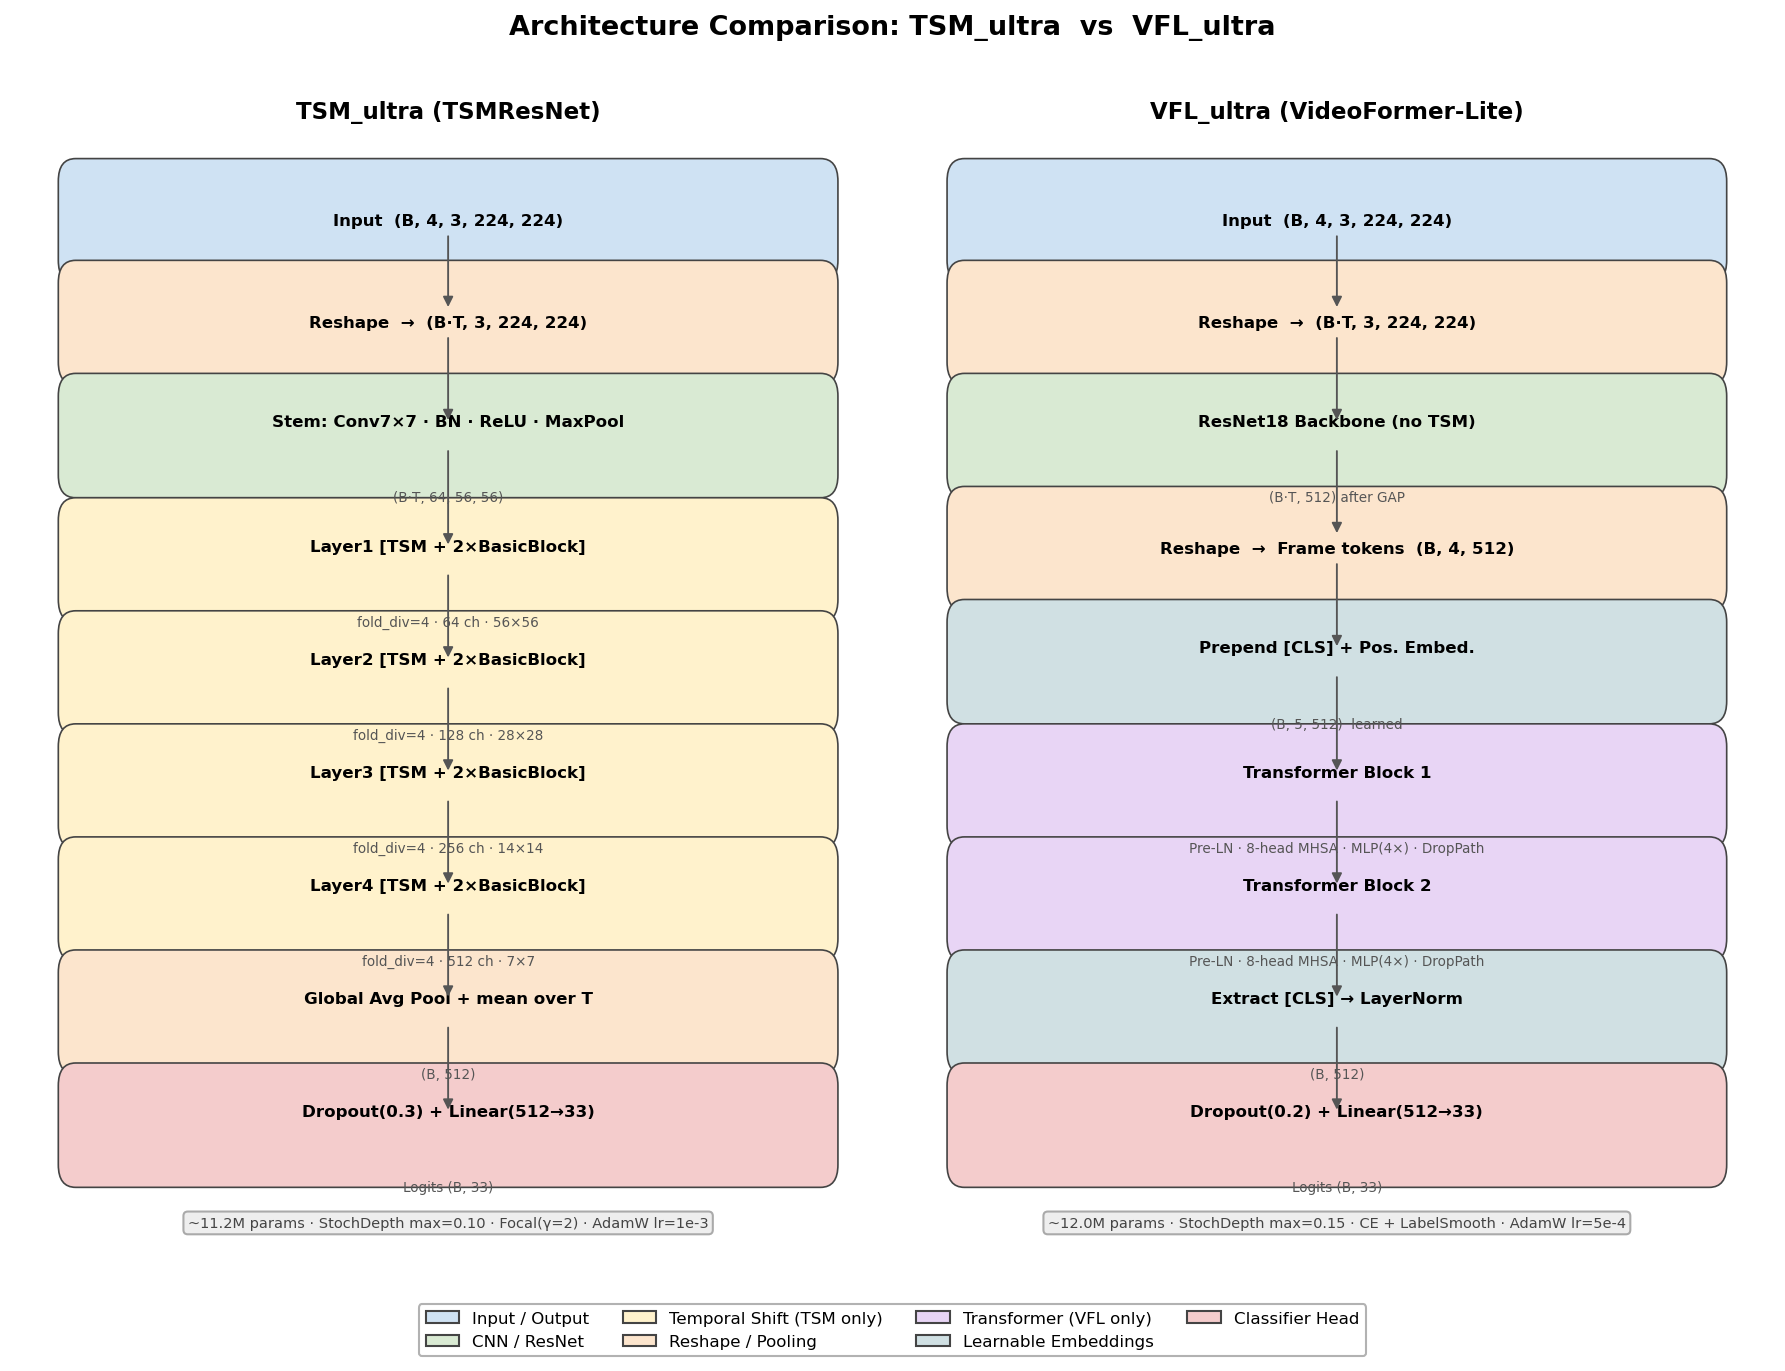
\includegraphics[width=\linewidth]{arch_comparison.png}
  \caption{The two complementary Track~A temporal mechanisms. \textbf{TSM} mixes
  time \emph{locally} via parameter-free channel shifts in every ResNet block;
  \textbf{VideoFormer-Lite} mixes time \emph{globally} via \texttt{[CLS]}-token
  attention over the four frame tokens. Their orthogonal biases drive the
  ensemble gain (Sec.~\ref{sec:trackA}).}
  \label{fig:arch}
\end{figure}

\begin{figure}[h]
  \centering
  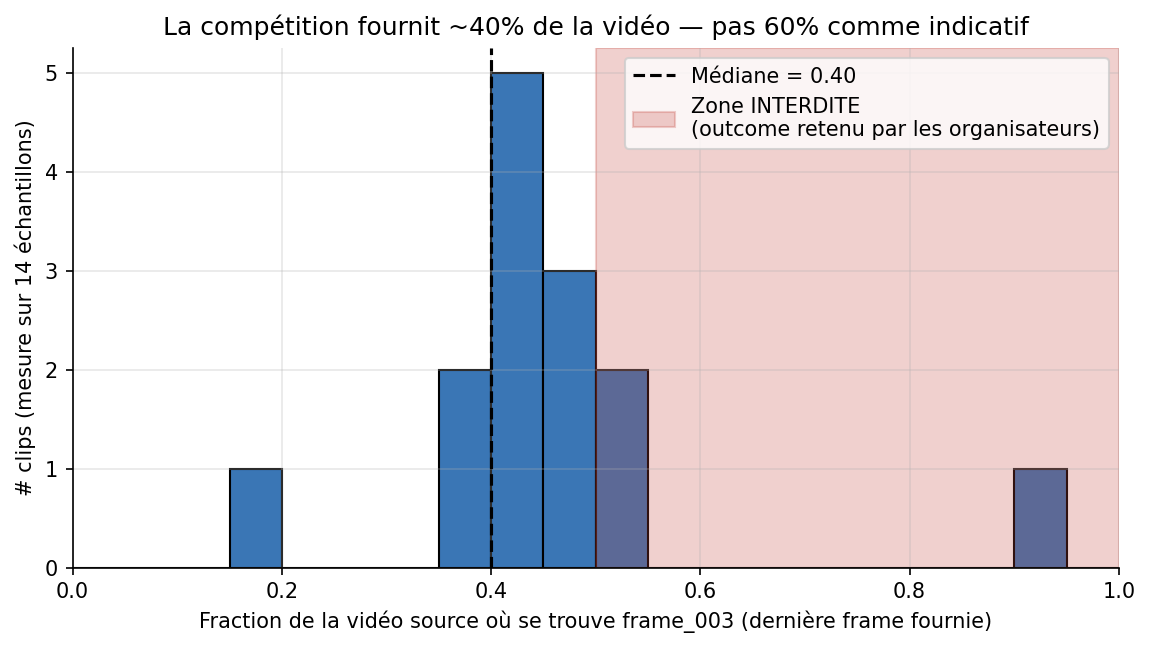
\includegraphics[width=\linewidth]{fig01_per_model_accuracy.png}
  \caption{Per-model \texttt{val\_dir} top-1/top-5 (Track~A). Correcting the
  frame count (TSM-Ultra$\rightarrow$TSM-Ultra-v2) is the single largest
  per-model jump; the ResNet-50/$T{=}8$ scale-up regresses
  (Sec.~\ref{sec:results}).}
  \label{fig:permodel}
\end{figure}

\begin{figure}[h]
  \centering
  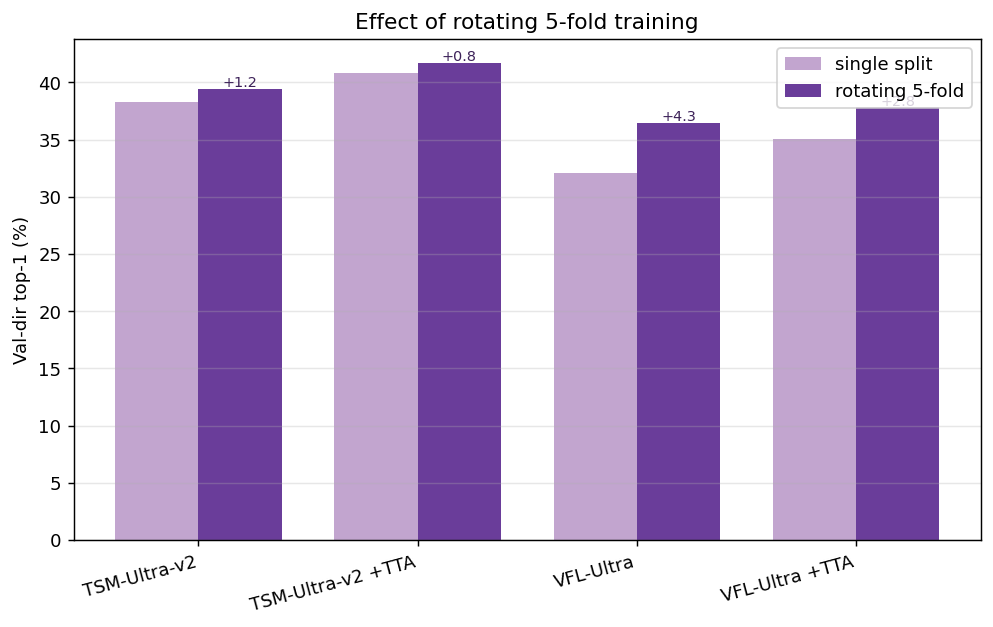
\includegraphics[width=\linewidth]{fig04_ensemble.png}
  \caption{Track~A ensemble vs.\ its components. Log-softmax late fusion of two
  TSM variants and one VFL variant (all +TTA) exceeds the best single model by
  $+2.35$\,pp top-1, reaching $44.03\%$ \texttt{val\_dir}.}
  \label{fig:ensemble}
\end{figure}

\begin{figure}[h]
  \centering
  
\includegraphics[width=\linewidth]{fig11_leave_one_out.png}
  \caption{Track~A leave-one-out study (\texttt{val\_dir} top-1). All three
  members are necessary; the weakest standalone model (VFL) still adds value
  through error decorrelation (Table~\ref{tab:loo}).}
  \label{fig:loo}
\end{figure}

\begin{figure}[h]
  \centering
  
\includegraphics[width=\linewidth]{fig02_tta_effect.png}
  \caption{Effect of 10-crop spatial TTA on Track~A models. TTA adds
  ${\sim}1$\,pp on the strongest checkpoint and is essential at the ensemble
  level, where independent random errors from different crops average out
  (Sec.~\ref{sec:trackA}).}
  \label{fig:tta}
\end{figure}

\begin{figure}[h]
  \centering
  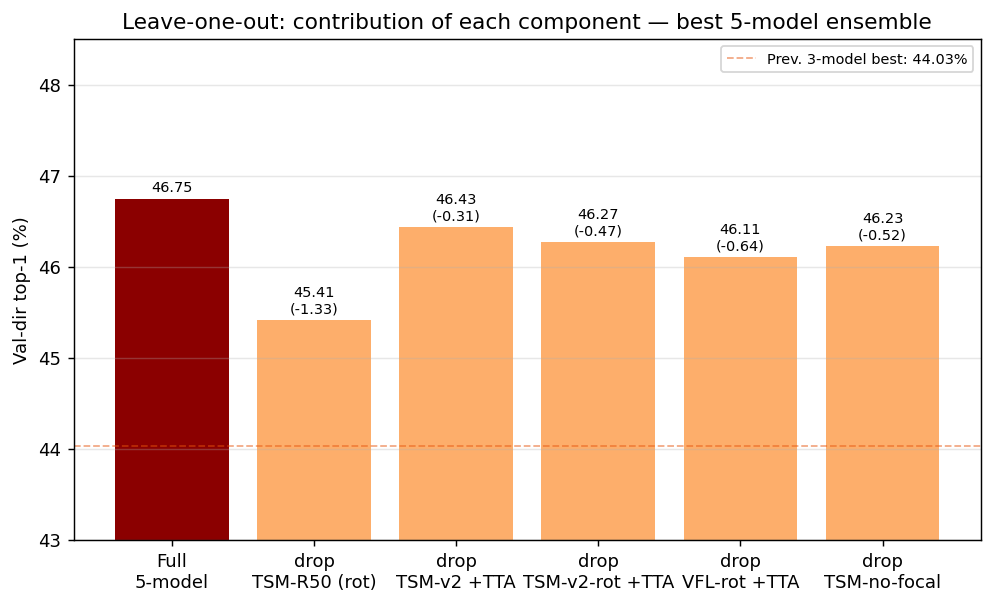
\includegraphics[width=\linewidth]{fig12_tta_directional_tradeoff.png}
  \caption{TTA directional-class trade-off. Horizontal-flip TTA improves most
  classes but hurts a few direction-encoded ones
  (\emph{Pulling left$\rightarrow$right} vs.\ \emph{right$\rightarrow$left})
  even after the flip-aware logit remap, because mirror evidence is
  intrinsically ambiguous when motion is short.}
  \label{fig:ttatradeoff}
\end{figure}

\begin{figure}[h]
  \centering
  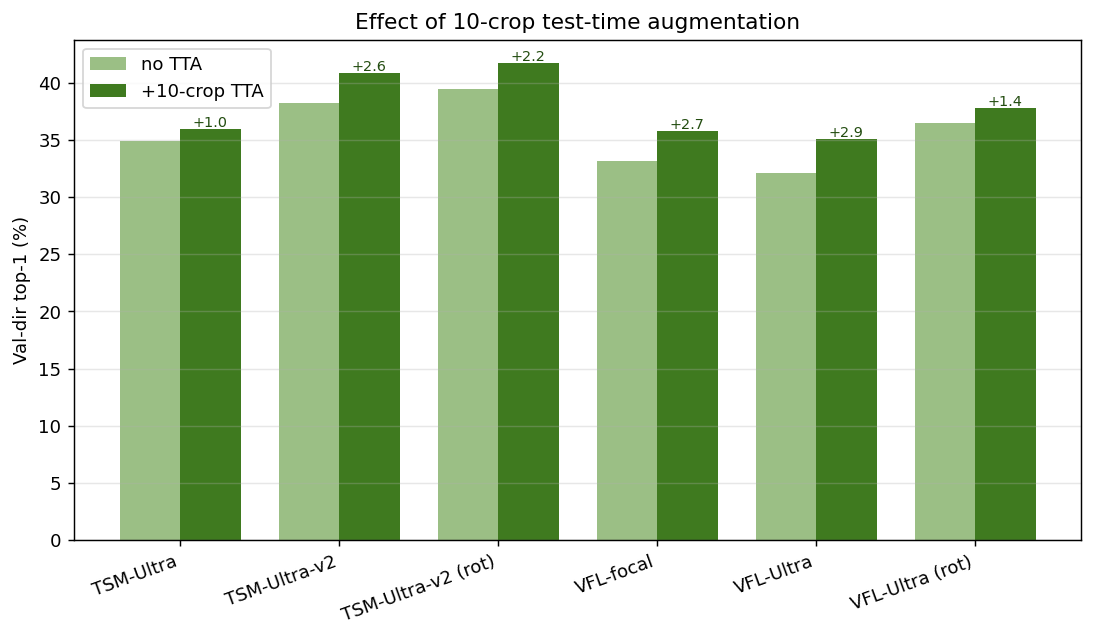
\includegraphics[width=\linewidth]{fig03_rotating_effect.png}
  \caption{Rotating-fold training. Re-training the strongest checkpoint on
  every train/val fold yields snapshots that share weights but disagree on the
  boundary, contributing uncorrelated errors that the log-softmax ensemble
  exploits (Sec.~\ref{sec:trackA}).}
  \label{fig:rotating}
\end{figure}

\begin{figure}[h]
  \centering
  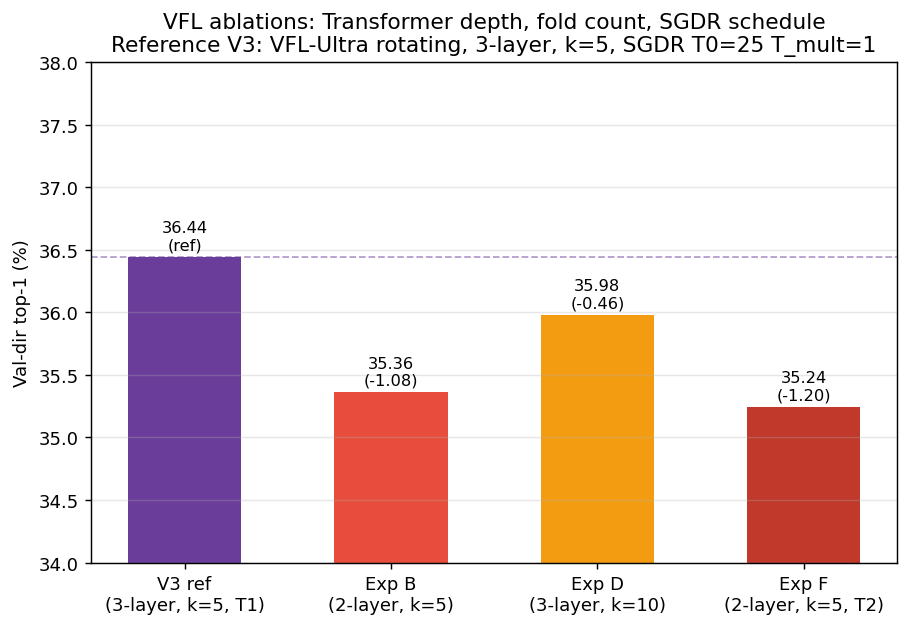
\includegraphics[width=\linewidth]{fig18_backbone_r18_vs_r50.png}
  \caption{Backbone scale-up does not compensate for corrupted temporal input.
  Switching from ResNet-18/$T{=}4$ to ResNet-50/$T{=}8$ regresses internal
  validation by ${\sim}8$\,pp because the larger $T$ triggers frame
  interpolation (Sec.~\ref{sec:trackA}).}
  \label{fig:backbone}
\end{figure}

\begin{figure}[h]
  \centering
  
\includegraphics[width=\linewidth]{A_kaggle_journey.png}
  \caption{Track~B honest Kaggle progression. The discarded leaky submission
  ($0.81$, red) is plotted alongside every clean ensemble; each gain comes from
  adding architecturally distinct members, not from re-weighting. The dashed
  line marks the second-place public reference ($0.74$); the gap to it bounds
  what self-supervised pretraining + diverse ensembling buys us
  (Sec.~\ref{sec:results}, Table~\ref{tab:kaggle}).}
  \label{fig:kagglejourney}
\end{figure}

\begin{figure}[h]
  \centering
  
\includegraphics[width=\linewidth]{D_training_curves.png}
  \caption{V-JEPA progressive unfreezing + LLRD (Track~B internal val). Each
  phase warm-starts above the previous plateau: frozen probe ($0.55\!\to\!0.67$),
  then top-6 unfrozen + LLRD ($0.68\!\to\!0.71$), then full encoder
  ($0.70\!\to\!0.73$), then pseudo-label retrain ($0.72\!\to\!0.74$). The
  staircase pattern is the visual signature that LLRD has preserved each
  phase's feature geometry (Sec.~\ref{sec:trackB}).}
  \label{fig:vjepacurves}
\end{figure}

\begin{figure}[h]
  \centering
  
\includegraphics[width=\linewidth]{E_frame_position_histogram.png}
  \caption{Where shipped \texttt{frame\_003} sits in the source SSv2 clip
  (fraction). The dashed line at $0.40$ is the median end-of-window; the shaded
  region $[0.50,1.00]$ is the withheld outcome --- our re-extraction is
  hard-bounded to the un-shaded region (Sec.~\ref{sec:integrity}).}
  \label{fig:framehist}
\end{figure}

\begin{figure}[h]
  \centering
  
\includegraphics[width=\linewidth]{B_ensemble_size_vs_score.png}
  \caption{Track~B Kaggle vs.\ ensemble size. Returns from adding diverse
  honest members are still positive at $n{=}14$; at $n{=}6$, dropping K400
  + TSM \emph{hurts} despite their lower individual scores, because their
  uncorrelated errors disappear from the average
  (Table~\ref{tab:strategy}).}
  \label{fig:enssize}
\end{figure}

\begin{figure}[h]
  \centering
  
\includegraphics[width=\linewidth]{I_learned_weights_collapse.png}
  \caption{Learned ensemble weights collapse onto the two strongest members
  (${\sim}82\%$ of mass on \texttt{large\_attempt1\_top2} and
  \texttt{ssv2\_top1}), effectively zeroing K400 contributions. This is exactly
  why a learned weighting fails to beat uniform: it discards the very
  decorrelation signal that diverse weaker members provide
  (Sec.~\ref{sec:results}).}
  \label{fig:learnedw}
\end{figure}

\begin{figure*}[h]
  \centering
  
\includegraphics[width=0.95\textwidth]{fig05_per_class_f1.png}
  \caption{Per-class F1 (ensemble, \texttt{val\_dir}). Directional single-object
  motions score highest; ``pretending'' and direction-ambiguous classes score
  lowest (Sec.~\ref{sec:failure}).}
  \label{fig:perclass}
\end{figure*}

\begin{figure*}[h]
  \centering
  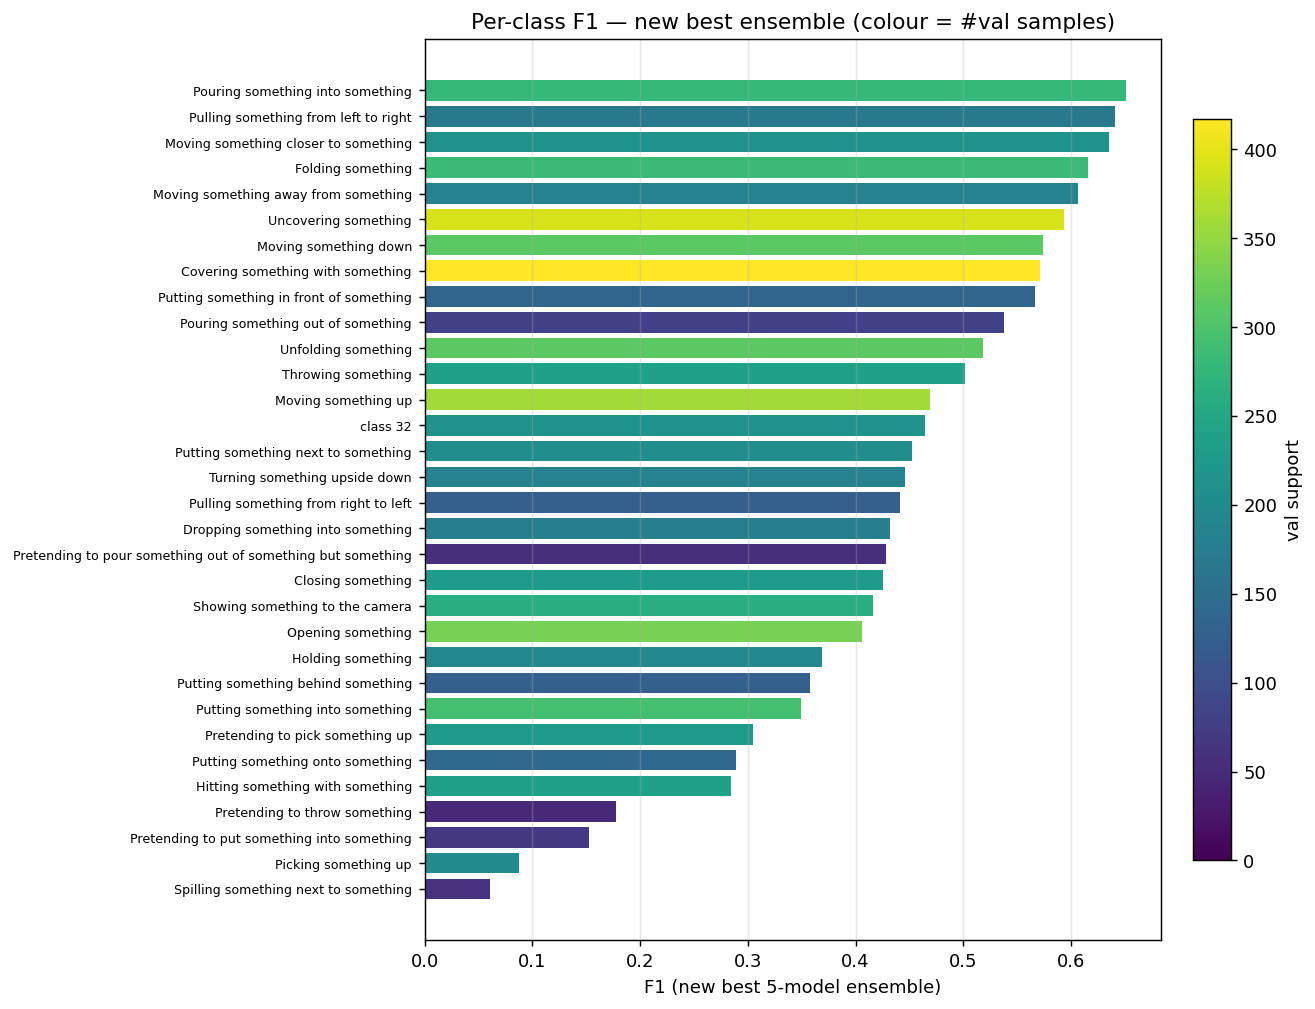
\includegraphics[width=0.95\textwidth]{fig06_confusion_matrix.png}
  \caption{$33\times33$ confusion matrix (ensemble, \texttt{val\_dir}).
  Off-diagonal mass concentrates on semantically adjacent pairs (real vs.\
  pretended; fold vs.\ unfold; motion vs.\ \emph{holding}).}
  \label{fig:confmat}
\end{figure*}

\begin{figure*}[h]
  \centering
  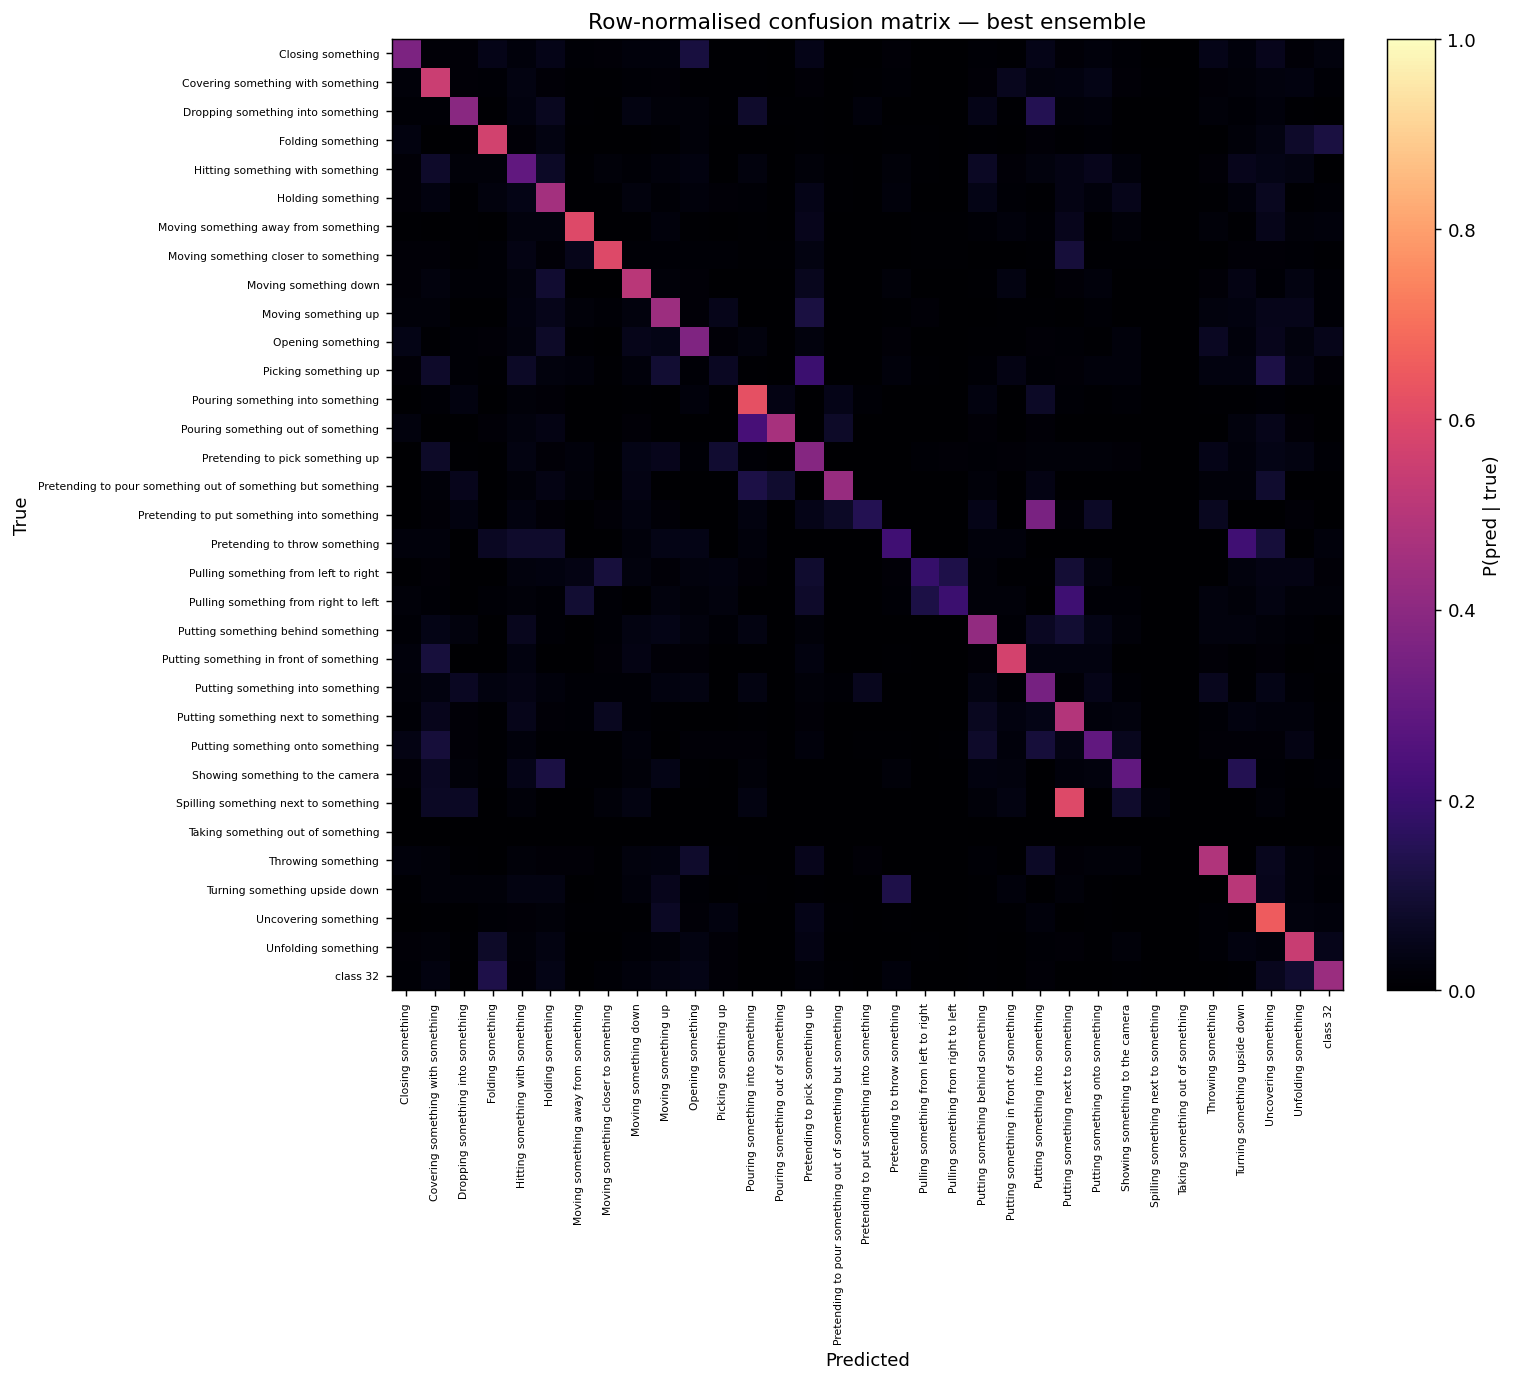
\includegraphics[width=0.95\textwidth]{fig07_confused_pairs.png}
  \caption{Most-confused class pairs. The dominant errors are intent (real vs.\
  pretended) and temporal-direction confusions (Sec.~\ref{sec:failure}).}
  \label{fig:pairs}
\end{figure*}

% =====================================================================
\clearpage
{\small
\bibliographystyle{ieeenat_fullname}
\bibliography{references}
}

\end{document}
